\documentclass[10pt,a4paper,reqno]{amsart}
%\documentclass[ a4paper,twoside, 11pt, titlepage]{amsart}
\usepackage{amsfonts,amsthm,latexsym,amsmath,amssymb,amscd,amsmath,epsf,morefloats}
\usepackage{placeins}
%,showlabels}
\usepackage{graphicx}
\usepackage{tikz}
%\extrafloats{100}

\newtheorem{Def}{Definition}
\newtheorem{Theorem}{Theorem}
\newtheorem{Lemma}{Lemma}
\newtheorem{Cor}{Corollary}
%\newtheorem{Conj}{Conjecture}
\newtheorem{Prop}{Proposition}
\newtheorem{Alg}{Algorithm}
\newtheorem{Rmk} {Remark}
\newtheorem{Ex} {Example}
\newtheorem{Prob} {Problem}
\newtheorem{Not}{Notation}
\newtheorem{theo+}           {Theorem}
\newtheorem{prop+}           {Proposition}
\newtheorem{coro+}           {Corollary}
\newtheorem{lemm+}           {Lemma}
\newtheorem{conjecture}      {Conjecture}
\theoremstyle{definition}
\newtheorem{defi+}           {Definition}
\newtheorem{problem}         {Problem}
\newtheorem{example}           {Example}

\theoremstyle{remark}
\newtheorem{rema+}           {Remark}

\newenvironment{theorem}{\begin{theo+}}{\end{theo+}}
\newenvironment{proposition}{\begin{prop+}}{\end{prop+}}
\newenvironment{corollary}{\begin{coro+}}{\end{coro+}}
\newenvironment{lemma}{\begin{lemm+}}{\end{lemm+}}
\newenvironment{remark}{\begin{rema+}}{\end{rema+}}
\newenvironment{definition}{\begin{defi+}}{\end{defi+}}
\newenvironment{notation}{\begin{not+}}{\end{not+}}




\newcommand{\Slut}{$\quad\Box$}
\newcommand{\Skip}{\smallskip\flushleft}
\newcommand{\Dim}{\textrm{dim}}
\newcommand{\Deg}{\textrm{deg}}
\newcommand{\Det}{\textrm{det}}
\newcommand{\al}{\alpha}
\newcommand{\bet}{\beta}
\newcommand{\Ups}{\Upsilon}
\newcommand{\Tak}{\hat{\alpha}_{i}}
%\newcommand {\bC} {\mathbb C}
%\newcommand {\bR} {\mathbb R}
%\newcommand {\D} {\mathcal D}
\newcommand {\CC}{\mathcal C}
\newcommand {\DD} {\mathbf D}
\newcommand {\bCP} {\mathbb {CP}}
\newcommand{\Pkt}{\textrm{.}}
\newcommand{\Kma}{\textrm{,}}
\newcommand {\Ga} {\Gamma}
\newcommand {\ga} {\gamma}
\newcommand {\eps} {\epsilon}
\newcommand {\de} {\delta}
\newcommand \dq {\mathfrak d(z)}
\newcommand \dqn {\mathfrak d_n(z)}
\newcommand \dd {\mathfrak d}
\newcommand\pa {\partial}
\newcommand \alij{\alpha_i^{(j)}}
\newcommand{\ze}{\zeta}
\newcommand{\la}{\lambda}
\newcommand{\La} {\Lambda}
\newcommand{\Si}{\Sigma}
\newcommand{\si}{\sigma}
\newcommand{\bC}{\mathbb C}
\newcommand{\bR}{\mathbb R}
\newcommand{\bN}{\mathbb N}
\newcommand{\bZ}{\mathbb Z}
\newcommand{\bD}{\mathbb D}
\newcommand{\A}{\mathcal A}
\newcommand{\D}{\mathcal D}
\newcommand{\C}{\mathcal C}
\newcommand{\Z}{\mathcal Z}
\newcommand{\N}{\mathcal N}
\newcommand{\NN}{\mathbb N}
\newcommand{\cS}{\mathcal S}
\newcommand{\RR}{\mathbb{R}}
\newcommand {\wA} {\widetilde {\mathcal A}}
\newcommand{\EE}{\mathcal{E}}
\newcommand \bL {\bold L}
\newcommand{\meas}{{\rm meas}\,}
\newcommand{\Mod}{{\rm mod}\,}
\newcommand{\diam}{{\rm diam}\,}
\newcommand{\dist}{{\rm dist}\,}
\newcommand{\Area}{{\rm area}\,}
\newcommand{\be}{\begin{equation}}
\newcommand{\ee}{\end{equation}}
\newcommand{\bl}{\begin{lemma}}
\newcommand{\el}{\end{lemma}}
%\newtheorem{theorem}{Theorem}
%\newtheorem{lemma}{Lemma}
%\newtheorem{corollary}{Corollary}
\newtheorem{theo}{Theorem}
%\newtheorem{conjecture}{Conjecture}
\newtheorem{lemmaA}{Lemma}
\newcommand{\blemmaA}{\begin{lemmaA}}
\newcommand{\elemmaA}{\end{lemmaA}}
%\newtheorem{proposition}{Proposition}
\newcommand{\bprop}{\begin{proposition}}
\newcommand{\eprop}{\end{proposition}}
%\newtheorem{definition}{Definition}

\newtheorem{fig}{Box for Figure}
\renewcommand{\thetheo}{\Alph{theo}}
\renewcommand{\theequation}{\thesection.\arabic{equation}}
\renewcommand{\thelemmaA}{\Alph{lemmaA}}
\renewcommand{\thefigure}{}  %{\thesection.\arabic{equation}}
%\mag1200
\newcommand{\bt}{\begin{theorem}}
\newcommand{\et}{\end{theorem}}
\newcommand{\bc}{\begin{corollary}}
\newcommand{\ec}{\end{corollary}}
\newcommand{\bcon}{\begin{conjecture}}
\newcommand{\econ}{\end{conjecture}}
\newcommand{\ep}{\varepsilon}
\newcommand{\ph}{\varphi}
\newcommand{\va}{\varphi}
\newcommand{\cA}{{\cal{A}}}
%\newcommand{\al}{\alpha}
%\newcommand{\th}{\theta}
%\newcommand{\ga}{\gamma}
\newcommand{\Res}{{\rm{Res}}}
\newcommand{\CU}{{\overline{\U}}}
\newcommand{\U}{{\Bbb U}}
\newcommand{\II}{\int\!\!\int}
%\newcommand{\D}{{\cal D}}
%\newcommand{\DD}{{\mathbb{D}}}
\newcommand{\e}{\varepsilon}
\newcommand{\Om}{\Omega}
\newcommand{\om}{\omega}
\newcommand{\UH}{{\Bbb {H}}}

\newcommand{\Ha}{{\cal H}}
%\newcommand{\C}{{\Bbb C}}
%\newcommand{\CC}{{\overline{\C}}}
\newcommand{\R}{{\Bbb R}}
\newcommand{\T}{{\Bbb T}}
%\newcommand{\A}{{\cal A}}
\newcommand{\F}{{\cal F}}
\newcommand{\CR}{{\overline{\R}}}
\newcommand{\supp}{\operatorname{supp}}
\newcommand{\locint}{L^1_{loc}}

\def\newop#1{\expandafter\def\csname #1\endcsname{\mathop{\rm
#1}\nolimits}}

\newop{slc}
\newop{sign}
\newop{mdeg}

\renewcommand{\figurename}{Fig\hspace{-1mm}}












\begin{document}

\thispagestyle{empty}

{\Large{\textbf{Title:}}} {\large{Optimal Obstacle Problems: The
case of Harmonic Measure.}}

\bigskip


                 \centerline{{\Large{\textbf{Abstract}}}}
\medskip

\noindent %
Suppose we are interested in solutions $u$ of a \textbf{Boundary
Value Problem }on a domain $D$. We suppose further that a domain
$D$ is changed by inserting into $D$ an \emph{``obstacle"} $E$
from some class $\mathcal{E}=\{E\}$ where each obstacle $E$
carries its own boundary data. Then the \textbf{Optimal Obstacle
Problem} is to find an obstacle $E_0\in \mathcal{E}$ which
distorted the original solution $u$ as minimally as possible.

The main goal of my talk is to discuss the Optimal Obstacle
Problem for Harmonic Measures. More precisely, we will consider
the following problem.



 Let $D$ be a domain on $\mathbb{C}$ and let $E$ be a Borel set on
$\partial D$. Then $\omega(z,E,D)$ will denote the harmonic
measure of $E$ with respect to $D$; i.e. $\omega(z,E,D)$ is the
Perron solution to the Dirichlet problem in $D$ with boundary
values $1$ on $E$ and $0$ on $E'=\partial D\setminus E$. If $E$ is
a closed set on $\overline{\mathbb{C}}$ and $z\in D\setminus E$,
then $\omega(z,E,D)$ will denote the harmonic measure of the set
$E\cap\partial(D_z)$ with respect to the connected component $D_z$
of $D\setminus E$, which contains $z$. The harmonic measure can be
thought as the steady-state distribution of heat on $D$ created by
the heating element $E$.

 Let $A=\{a_1,\ldots,a_n\}$ and $B=\{b_1,\ldots,b_m\}$ be
two disjoint sets of distinct points in $D$. Let
${\mathcal{L}}_{A,B}(D)=\{L\}$ be the family of all  sets $L$ in
$\overline{D}$ of the form $L=\cup_{k=1}^n l_k$, where $l_k$ is a
continuum in $\overline{D}\setminus B$ connecting $a_k$ and
$\partial D$. Let $\omega_L(z)=\omega(z,L,D)$. Let
$F(x_1,\ldots,x_n)$ be a continuous real-valued function
increasing in each variable.

\smallskip

\noindent %
 \textbf{Obstacle problem. } %
 The obstacle problem on the
harmonic measure on $D$ for the function $F$ and sets $A$ and $B$
is to
find the infimum %
$$
 \label{1.1} \inf F(\omega_L(b_1),\ldots,\omega_L(b_m)), %
$$  %
taken over all $L\in {\mathcal{L}}_{A,B}(D)$ and identify all
\textit{obstacles} $L$ in ${\mathcal{L}}_{A,B}$ extremal for this
problem.
%\end{problem}

One particular goal of this talk is to discuss solution of the
obstacle problem in one of the simplest non-trivial cases, when
$D$ is the unit disk $\mathbb{D}=\{z:\, |z|<1\}$, $B=\{0\}$, and
$A=\{-r,r\}$ with some $0<r<1$. In this case, the problem can be
stated as follows.

\noindent %
\textbf{Obstacle problem for two heating elements.} \label{Problem 1.1} %
For fixed $r\in (0,1)$, find %the infimum%
$$ %\be \label{1.2} %
m(r)=\inf \omega_L(0), %
$$ %\ee %
taken over all sets $L=l_1\cup l_2$, where $l_1$ connects $r$ with
$\mathbb{T}=\partial \mathbb{D}$ and $l_2$ connects $-r$ with
$\mathbb{T}$ and identify all extremal obstacles. %
%\end{problem} %

\FloatBarrier


\begin{figure}
\centering %
%\hspace{-4.3cm} %
\begin{minipage}{0.60\linewidth}
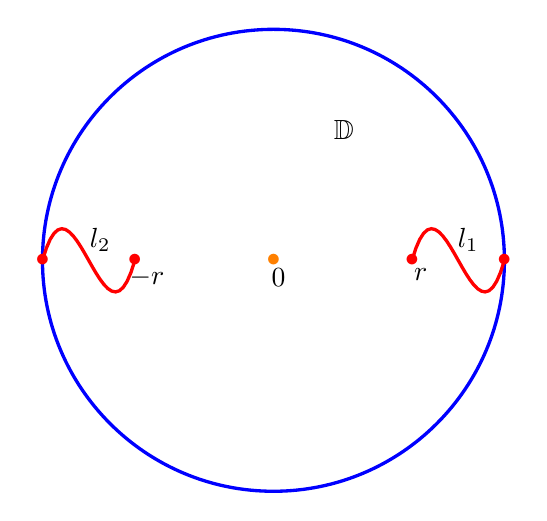
\begin{tikzpicture}
    [inner sep=1mm,
     place/.style={circle,draw=blue!50,
     fill=blue!20,thick},
     scale=2.2]%


%\begin{minipage}{0.60\linewidth}
%\begin{tikzpicture}
%    [inner sep=1mm,
%     place/.style={circle,draw=blue!50,
 %    fill=blue!20,thick},
  %   scale=3]%


\draw [blue, very thick](0,0) circle (4/3); %
\node at (0.8,0) [red] {$\bullet$}; %
\node at (4/3,0) [red] {$\bullet$}; %
\node at (-4/3,0) [red] {$\bullet$}; %
\node at (0.85,0) [below] {$r$};
\node at (-0.8,0) [red] {$\bullet$}; %
\node at (-0.73,0) [below] {$-r$};

\node at (1.125,0) [above] {$l_1$};

\node at (-1,0) [above] {$l_2$};

\node at (0,0) [orange,very thick] {$\bullet$}; %
\node at (0.03,0) [below] {$0$};

\node at (0.3,0.75) [right] {$\mathbb{D}$};




 \draw [red, very thick] plot[domain=4/5:4/3] ({(\x)},{(25*(\x-4/5)*(\x-16/15)*(\x-4/3))});

 \draw [red, very thick] plot[domain=4/5:4/3] ({(-\x)},{(-25*(\x-4/5)*(\x-16/15)*(\x-4/3))});
 \end{tikzpicture}

 \medskip

 \center{Round stove with two heating elements.\ \ \ \ \ \ \ \ \ \ \ }
\end{minipage}





%\caption{Round stove with obstacles.}
%\label{fig4}
\end{figure}




\end{document}
